% ****** Start of file apssamp.tex ******
%
%   This file is part of the APS files in the REVTeX 4.2 distribution.
%   Version 4.2a of REVTeX, December 2014
%
%   Copyright (c) 2014 The American Physical Society.
%
%   See the REVTeX 4 README file for restrictions and more information.
%
\documentclass[%
reprint,
amsmath,amssymb,
aps,
floatfix,
]{revtex4-2}

\usepackage{graphicx}
\usepackage{dcolumn}
\usepackage{bm}
\usepackage{natbib}
\usepackage{subcaption}
\usepackage{placeins}
\usepackage{amsmath}
\usepackage{booktabs}
\begin{document}
	
	\preprint{APS/123-QED}
	
	\title{Quantitative analysis of the complexity of dynamical systems}
	\thanks{A footnote to the article title}
	
	\author{Ann Author}
	\altaffiliation[Also at ]{Physics Department, University of Dhaka.}
	\author{Second Author}
	\email{Second.Author@institution.edu}
	\affiliation{%
		Authors' institution and/or address\\
		This line break forced with \textbackslash\textbackslash
	}
	
	\collaboration{MUSO Collaboration}
	
	\author{Charlie Author}
	\homepage{http://www.Second.institution.edu/~Charlie.Author}
	\affiliation{
		Second institution and/or address\\
		This line break forced
	}%
	\affiliation{
		Third institution, the second for Charlie Author
	}%
	\author{Delta Author}
	\affiliation{%
		Authors' institution and/or address\\
		This line break forced with \textbackslash\textbackslash
	}
	
	\collaboration{CLEO Collaboration}
	
	\date{\today}
	
	\begin{abstract}
		Abstract
		\begin{description}
			\item[Usage] Secondary publications and information retrieval purposes.
			\item[Structure] The paper presents a comprehensive framework for quantifying complexity in chaotic systems.
		\end{description}
	\end{abstract}
	
	\maketitle
	
	\section{\label{sec:level1}Introduction}
	
	The Lorenz attractor arises from a simplified model of atmospheric convection developed by Edward N. Lorenz in 1963. It is also studied in information theory, complexity science, and geometric analysis.\\
	It is given by three coupled differential equations. The solution to these equations traces a beautiful butterfly-shaped trajectory in xyz-space. By simply observing this trajectory, we recognize that it is not a simple system. Yet quantifying this complexity remains difficult. There are some defined ways to measure complexity such as Kolmogorov complexity, López-Ruiz-Mancini-Calbet (LMC) complexity, etc. 
	We can compute existing complexity measures, but this immediately raises a vital question: "Are these measures even sufficient for capturing the true complexity of this system? If not, what alternative approach can we discover?"
	If we succeed in establishing a meaningful new quantity for measuring complexity, it must carry genuine physical significance.\\
	Simultaneously, we can explore other measurements that can describe the system like entropy, as entropy in general quantifies the unpredictability and the lack of information. One finds several entropies such as Boltzmann entropy, Shannon entropy, Kolmogorov–Sinai entropy (KS entropy), approximate entropy, sample entropy, permutation entropy, and many more. With so many entropy definitions available, we must ask: Do all entropies tell the same story, or do they reveal fundamentally different aspects? Moreover, we could seek novel kinds of entropy that might describe this system more effectively.\\
	Furthermore, the Lorenz attractor is an example of deterministic chaos. The term deterministic chaos means that the system originates from a set of deterministic equations, yet produces behavior that is unpredictable in the long term although it is predictable in the short term. Given its chaotic nature, we might also calculate quantities like Lyapunov exponents, which explain how sensitive a dynamical system is to initial conditions, and multifractal spectrum (need to write why we use it), etc.\\
	Beyond dynamics, we may also look for geometric properties – extracted not only from the trajectory itself, but also from phase space, velocity space, and beyond. (need to write what kind of geometry we may find)\\
	In order to calculate all these, we have three time series (x, y, z). One may study them statistically or using information theory. In either case, each time series can be studied individually, but we must understand their interdependence. Therefore, these series demand mutual analysis.\\
	To uncover relationships between key quantities, we can employ tools like mutual information, transfer mutual information, etc. Even though the system is chaotic, we can search for periodicity using autocorrelation which measures how a signal relates to itself over time and Higuchi Fractal Dimension for estimating fractal dimension.  Moreover, we need to understand how we can find geometric properties from these time series.
	In order to understand it we could try to find if there is any conserved quantity as energy, work etc. However as it is a bound orbit we might think if there exist any homoclinic or heteroclinic orbit. If they exist how many of them are there. 
	\section{Literature Survey}
	\subsection{Shannon Entropy}
	Shannon entropy (SE), introduced by Claude Shannon (site) that quantifies the average uncertainty of a random variable. For a discrete variable $X$ with outcome ${x_i}$, is defined as:
	
	\begin{equation}
		H(X) = -\sum_{i} p(x_i) \log_2 p(x_i)
		\label{eq:shannon}
	\end{equation}
	where $p(x_i)$ is the probability of outcome $x_i$.where,
	\[
	H(X) \geq 0
	\]
	SE calculates the entropy of entropy of symbolic sequences. High SE indicates high chaoticity. However, SE ignores geometric structure. As a result same SE values can be arrived from geometrically different  structure. Besides it can not capture directional information flow.\\
	\subsection{Kolmogorov-Sinai Entropy}
	The Kolmogorov-Sinai (KS) entropy, introduced independently by Kolmogorov (1958) and Sinai (1959). It measure the rate of information production in deterministic dynamical systems which refers to the rate at which a system generates uncertainty about its future state. KS entropy is defined as:
	\begin{equation}
		h_u  = \operatorname*{sup}_{\mathcal{P}} \operatorname*{\lim}_{n \to \infty} \frac{1}{n} h(P_n)	
	\end{equation}
	\subsection{Rényi entropy}
	Rényi entropy [] is generalization of Shannon entropy which quantify uncertainty or randomness of a system using a parameter $\alpha$. For a discrete probability distribution $P = (p_1,p_2,...,p_k)$ this is defined as:
	\begin{equation}
		H_\alpha (P) = \frac{1}{1 - \alpha} \log (\sum_{i=1}^{k} p_{i}^{\alpha})
	\end{equation}
	R\'enyi entropy is particularly useful in analyzing where a single scaling entropy measure may not suffice []. 
	here:\\
	$\alpha \geq 0$\\ 
	$\alpha \neq 1$ (for $\alpha$ = 1, it converge to Shannon entropy)\\
	\subsection{Transfer Entropy}
	Transfer entropy (TE) [] quantifies the directional flow of information between two time series. It is widely used in chaos theory, neuroscience and complex system making it highly relevant for studying Lorenz attractor. For two time series $X$ and $Y$ the transfer entropy from Y to X is:
	\begin{equation}
		T_{Y\to X} = \sum p(x_{t+1}, x_{t}^{(k)}, y_{t}^{(k)}) \log\left( \frac{p(x_{t+1} \mid x_{t}^{(k)}, y_{t}^{(k)})}{p(x_{t+1} \mid x_{t}^{(k)})} \right)
	\end{equation}
	TE can identify dominant driving variable. It also detects dynamic causation. Besides Lyapunov exponents [] measure local instability and KS entropy calculates global unpredictability but not coupling structure but TE complements these by quantifying information transfer pathway.
	\subsection{Permutation Entropy}
	Permutation entropy (PE), introduced by Bandt and Pompe in 2002 []. It is a simple method for quantifying complexity. Unlike traditional entropy PE calculates the unpredictability or randomness of a signal by analyzing the ordinal patterns of its values. PE is broadly use is the study of chaotic system.
	\begin{equation}
		H_{PE} = -\sum_{i} P(\pi_i) \log P(\pi_i)
	\end{equation}
	Here $P(\pi_i)$ is the probability of pattern $\pi_i$.\\
	High PE refers irregular behavior and low PE indicates deterministic nature. PE ignores amplitude as a result weighted permutation entropy is used. Moreover, it can not handle equal values is neighborhood. For this reason we can use weighted permutation entropy.
	\subsection{Weighted Permutation Entropy}
	Weighted Permutation Entropy (WPE) is an advanced variant of PE. Unlike PE it includes amplitude information into complexity analysis. WPE is a powerful tool for chaotic system like Lorenz attractor as both ordinal patterns and amplitude variations play critical role here.
	\begin{equation} 
		H_{WPE} = -\sum_{\pi} p_w(\pi) \ln p_w (\pi)
	\end{equation} 
	
	Where $p_w(\pi)$ is weighted probability of observing an ordinal pattern $\pi$ in a time series.\\
	(need to make sure the eq for wpe)\\
	where $w_i$ is variance $w_i = \frac{1}{m} \sum_{k=1}^{m} (x_{i+(k-1)\tau} - \overline{x}_i) $
	\subsection{Mutual Information}
	Mutual Information (MI) measures the nonlinear dependence between two random variables. It estimates how much knowing one variable reduces uncertainty about another. In the context of dynamical systems , it's used to study interdependence between different time series or system components. Let $X$ and $Y$ be two random variable and $p(x,y)$ ber joint probability and $p(x)$ and $p(y)$ be marginal probability. In that case MI is defined as:
	\begin{equation}
		I(X,Y) = \sum_{x\in X} \sum_{y\in Y} p(x,y) \log \frac{p(x,y)}{p(x)p(y)}
	\end{equation}
	It can also be interpreted as:
	\begin{equation}
		I(X,Y) = H(X) + H(Y) - H(X,Y)
	\end{equation}
	where $H(X)$, $H(Y)$ and $H(X,Y)$ and Shannon entropy of $X$, $Y$ and joint SE of $X$ and $Y$ respectively.
	\subsection{Higuchi Fractal Dimension}
	Higuchi Fractal Dimension (HFD) [] is an efficient way to estimate fractal dimention (FD) [] of a time series. It was introduced by T. Higuchi (1988). It gives a quantitative measure of complexity. Besides chaos analysis it is widely used in neuroscience and signal processing.\\
	need to finish it
	\subsection{Autocorrelation}
	Autocorrelation [] computes how much a signal correlates with a time-shifted or delayed version of  itself. It can be used for detecting periodicity and predictability by evaluating how its past values influence the future values of a time series.\\
	For a time series ${x_t}_{t=1}^N$ and lag $\tau$, autocorrelation $R(\tau)$ is:
	\begin{equation}
		R(\tau) = \frac{\sum_{t=1}^{N-\tau} (x_t - \overline{x}) (x_{t+\tau} - \overline{x})}{\sum_{t=1}^{N} (x_t - \overline{x})^2}
	\end{equation}
	Here range of $R(\tau) \in [-1,1]$ \\
	We can use it to find periodicity in Lorenz system. Furthermore, rapid decay of $R(\tau)$ indicates high chaos and slow decay of it refers predictability.\\
	\subsection{Homoclinic Orbit}
	Its a trajectory that starts and ends at the same saddle point.
	Which means it is said to be Homoclinic orbit if\\
	\begin{equation}
		\lim_{t\to -\infty} x(t) = x_0
	\end{equation}
	and
	\begin{equation}
		\lim_{t\to \infty} x(t) = x_0
	\end{equation}
	where $x_0$ is a saddle equilibrium.\\
	This types of orbits create a closed loop in phase space. Besides it is sensitive to perturbation as a result a tiny change destroy the orbit.
	\subsection{Heteroclinic Orbit}
	This types of trajectory connects two different saddle equilibria. It starts at a saddle point $x_a$ as $t\to-\infty$ and ends at another saddle $x_b$ as $t\to\infty$:
	\begin{equation}
		\lim_{t\to-\infty}x(t)= x_a	  and   \lim_{t\to\infty}x(t)= x_b
	\end{equation}
	It forms a bridge between two saddle points. However it is often seen in symmetric system.\\
	To find these types of orbits first we need to calculate the saddle equilibrias. we need to solve the values of $x$, $y$ and $z$ for $\dot{x}=0$, $\dot{y}=0$ and $\dot{z}=0$.\\
	after solving it we get,\\
	\begin{equation}
		(x,y,z) = (0,0,0)
	\end{equation}
	and
	\begin{equation}
		(x,y,z) = (\pm \sqrt{\beta(\rho -1)}, \pm \sqrt{\beta(\rho -1)}, \rho -1)
	\end{equation}
	\\
	Moreover, in order to find the work done on the particle firstly we calculate the expression for the acceleration by differentiating the the equation of this Lorenz system and for a unit mass particle we calculate the work on it.
	\begin{equation}
		a_x = \sigma(v_y - v_x)
		a_y = \gamma v_x + v_x z - v_z x +v_y
		a_z = v_x y + v_y x - \beta v_z
	\end{equation} 
	using these expression for acceleration and for $m=1$ we compute the work by
	\begin{equation}
		W= \int \vec{F} \cdot d\vec{s}
	\end{equation}
	if the work done on it reaches to any constant value over time then we can say this particle would stop after a time. However we can also check if the work is positive or negative.
	\subsection{\label{sec:citeref}Citations and References}
	
	
	\subsubsection{Citations}
	
	
	\paragraph{Syntax}
	
	
	\paragraph{The options of the cite command itself}
	
	
	\subsubsection{Example citations}
	
	
	\subsubsection{References}
	
	
	\subsubsection{Example references}
	
	
	
	
	\subsection{Footnotes}%
	
	\section{Methodology}
	To find the geometric properties of the Lorenz system, firstly, we take cross sections of the phase space as $p_x$ vs $x$, $p_y$ vs $p_z$ etc and observed them. We avoid terms like $p_x$ vs $y$. However, we also checked if the kinetic energy of the system is conserved or not. Since, for a system usually the total energy is conserved sometimes we therefore try to calculate the work on a unit mass particle. After this we summed and subtracted this from the kinetic energy to find if these results are constant. 
	we also try to find some average values like average of $x$, $v_x$ etc. Besides, for a range of parameter's value homoclinic and heteroclinic orbits are found. We took the values of $\rho$, $\sigma$ and $\beta$ to be [0,30] as the perameters are positive of lorenz system. With step 1, 29791 trajectories was examined for being homoclinic or heteroclinic or none of them. As these types of trajectories are vary rare we expected to find a few trajectories of these types.    \\
	As its known that for a straight line the $\ddot{\vec{r}}$ is zero and for a circle $\dot{\vec{r}}$ is zero for this reason dot product and cross product of these terms was calculated over time. If this terms converge it might be a property of the system.
	
	\section{Results and Discussion}
	If we analysis the slices of phase space we find that each of the 2D slices have some kind symmetry or anti-symmetry of the trajectory on that about a line. For different slices the lines are different. We believe that if it was possible to let the time goes for infinity one might find that each point on a bound space were covered. 
	\FloatBarrier
	\begin{figure}[htbp]
		\centering
		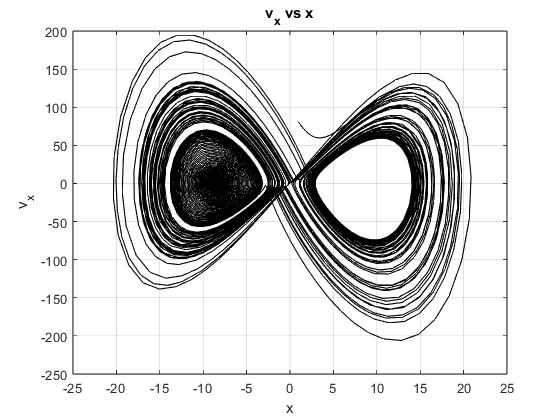
\includegraphics[width=0.8\linewidth]{v_x_vs_x.png}
		\caption{Phase Space: $v_x$ vs $x$}
		\label{fig:vx_x}
	\end{figure}
	
	\begin{figure}[htbp]
		\centering
		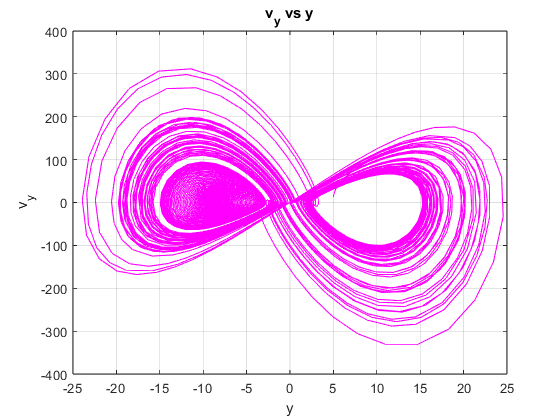
\includegraphics[width=0.8\linewidth]{v_y_vs_y.png}
		\caption{Phase Space: $v_y$ vs $y$}
		\label{fig:vy_y}
	\end{figure}
	
	\begin{figure}[htbp]
		\centering
		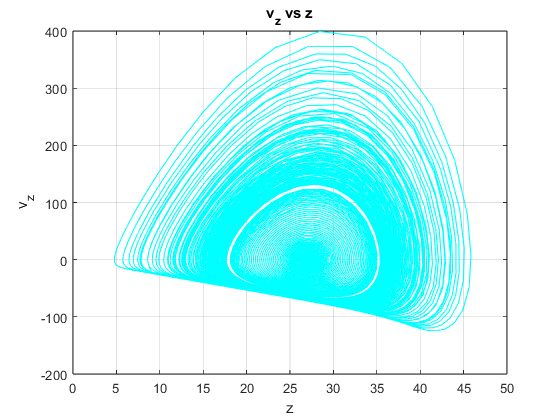
\includegraphics[width=0.8\linewidth]{v_z_vs_z.png}
		\caption{Phase Space: $v_z$ vs $z$}
		\label{fig:vz_z}
	\end{figure}
	
	\begin{figure}[htbp]
		\centering
		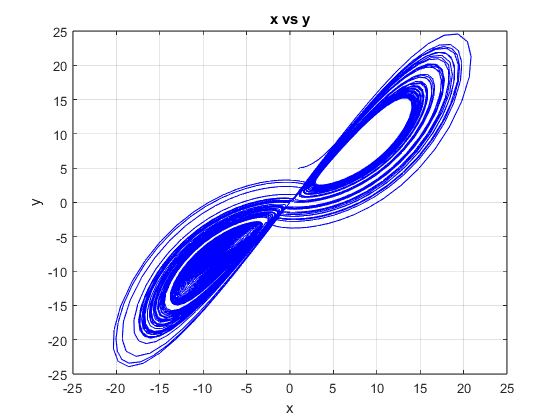
\includegraphics[width=0.8\linewidth]{y_vs_x.png}
		\caption{Position Space: $y$ vs $x$}
		\label{fig:y_x}
	\end{figure}
	
	\begin{figure}[htbp]
		\centering
		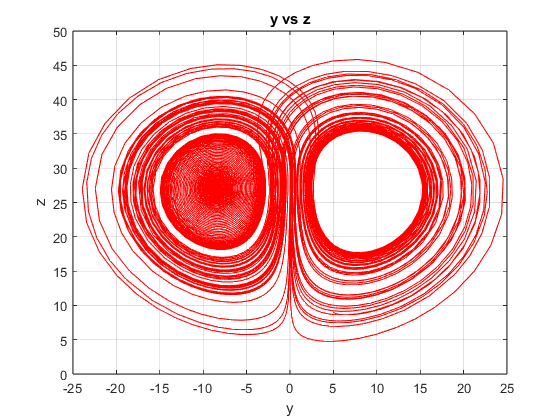
\includegraphics[width=0.8\linewidth]{z_vs_y.png}
		\caption{Position Space: $z$ vs $y$}
		\label{fig:z_y}
	\end{figure}
	
	\begin{figure}[htbp]
		\centering
		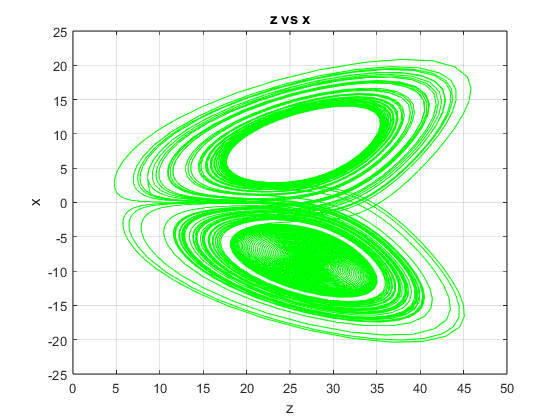
\includegraphics[width=0.8\linewidth]{x_vs_z.png}
		\caption{Position Space: $x$ vs $z$}
		\label{fig:x_z}
	\end{figure}
	
	\begin{figure}[htbp]
		\centering
		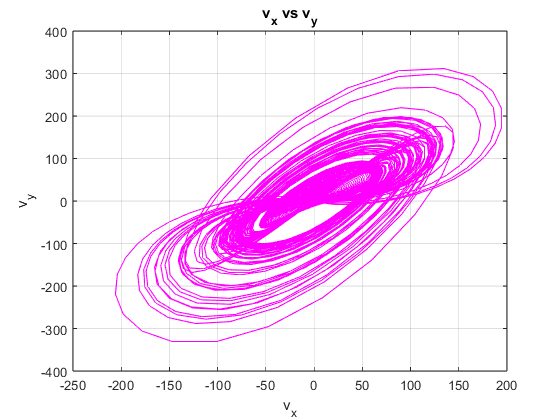
\includegraphics[width=0.8\linewidth]{vy_vs_vx.png}
		\caption{Velocity Space: $v_y$ vs $v_x$}
		\label{fig:vy_vx}
	\end{figure}
	
	\begin{figure}[htbp]
		\centering
		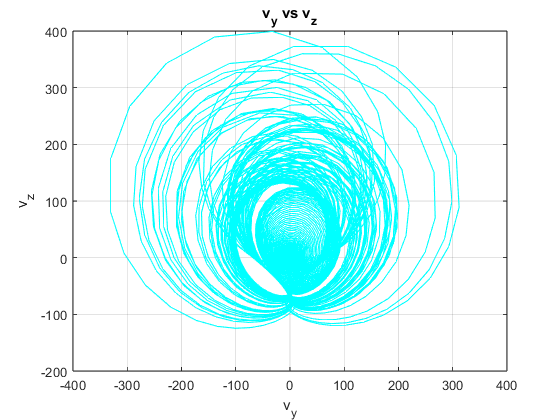
\includegraphics[width=0.8\linewidth]{vz_vs_vy.png}
		\caption{Velocity Space: $v_z$ vs $v_y$}
		\label{fig:vz_vy}
	\end{figure}
	
	\begin{figure}[htbp]
		\centering
		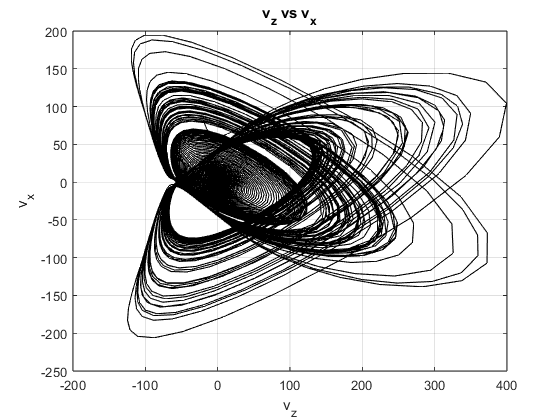
\includegraphics[width=0.8\linewidth]{vx_vs_vz.png}
		\caption{Velocity Space: $v_x$ vs $v_z$}
		\label{fig:vx_vz}
	\end{figure}
	
		
	\FloatBarrier
	
	None of kinetic energy, work and their summation or subtraction are conserved. Kinetic energy change rapidly over time which can be guessed from the trajectory of a particle in this system as its velocity change with no known pattern. Furthermore at some time the value of kinetic energy reaches near zero. This phenomena indicates that the particle sometimes falls into the attractor. When we simulate the motion this can be seen. Besides work by the particle is always negative. Which means some external agent is there to put any object into this type of motion. 
	\FloatBarrier
	\begin{figure}[htbp]
		\centering
		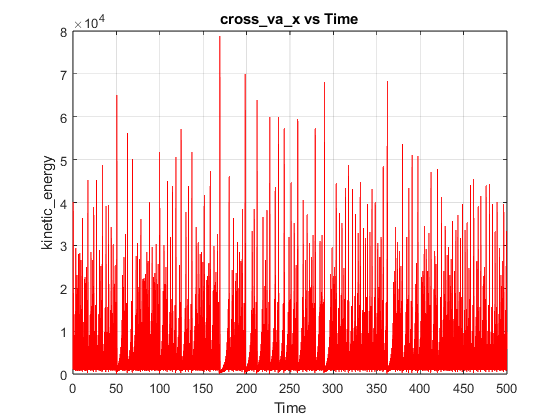
\includegraphics[width=0.8\linewidth]{kinetic_energy_plot.png}
		\caption{Kinetic Energy of the particle for$m=1$}
		\label{fig:kinetic_energy}
	\end{figure}
	\begin{figure}[htbp]
		\centering
		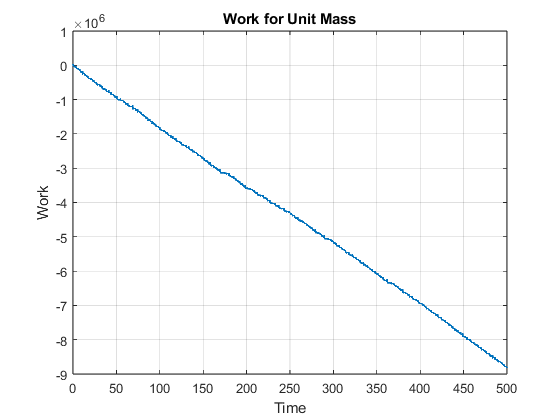
\includegraphics[width=0.8\linewidth]{work.png}
		\caption{Work by the particle}
		\label{fig:work}
	\end{figure}
	
	\FloatBarrier
	However $\langle x\rangle$, $\langle y\rangle$ and  $\langle z\rangle$ converge to some values. which is due to their nature of orbiting around some attractor. \\
	With step=1 for the values of $\rho$, $\sigma$ and $\beta$ in the range [0,30] we have found some values of $(\sigma, \beta, \rho )$ for which we get the homoclinic orbits and hetero clinic orbits.
	\FloatBarrier
	\begin{figure}[htbp]
		\centering
		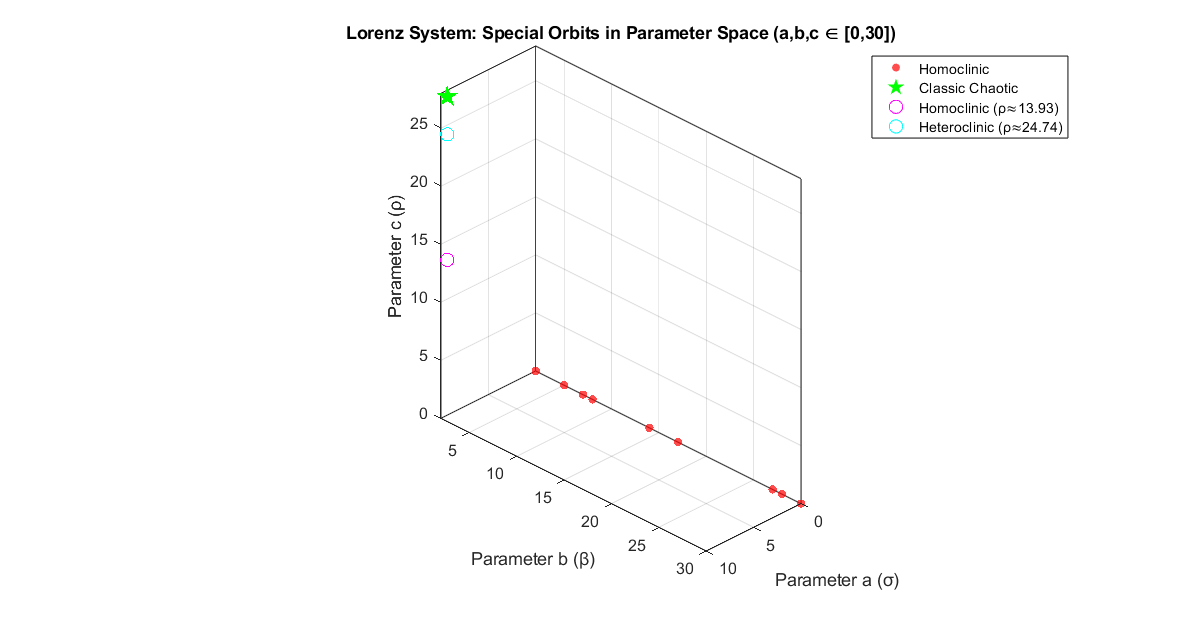
\includegraphics[width=1.5\linewidth]{homoclinic_heteroclinic_points.png}
		\caption{Parameters' value for Homoclinic and Heteroclinic orbits}
		\label{homoclini_heteroclinic}
	\end{figure}
	\FloatBarrier
	Neither the dot product nor the cross product of $\ddot{\vec{r}}$ and $\dot{\vec{r}}$ converged.\\
	Permutation entropy was measured by observing the pattern of 3 corresponding points. Initially, it was not stable, but after a period of time, this reached a constant value. As, at the beginning, the butterfly shape of the path is not obtained, we do not get the actual value of entropy. As we took three points, there are $3!$ patterns, and for this scenario the highest value to Permutation entropy one woukd get is $2.585$. But we did measure lower than that. If the trajectory was fully random we might get the highest value.
	\FloatBarrier
	\begin{figure}[htbp]
		\centering
		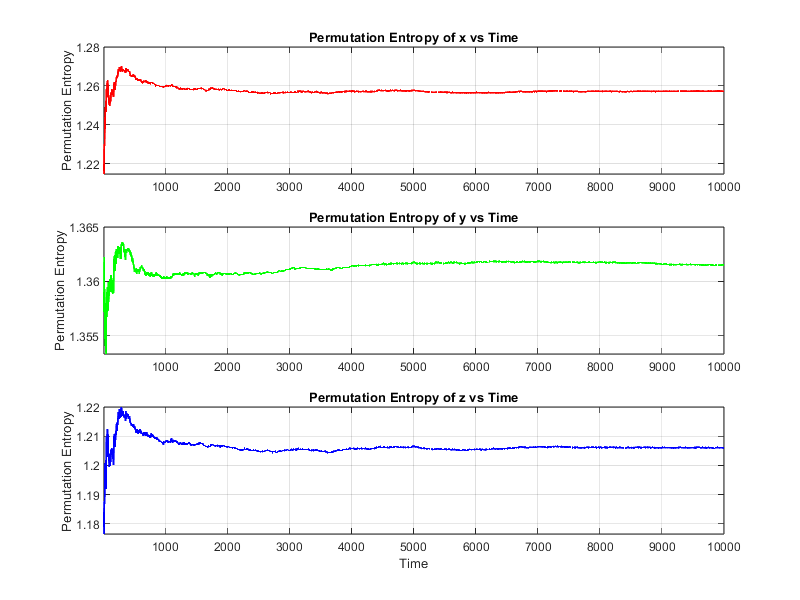
\includegraphics[width=0.8\linewidth]{PE_vs_time_x_y_z.png}
		\caption{Permutation Entropy}
		\label{PE_for_time_series}
	\end{figure}
	
	\FloatBarrier
	Similar behaviour was observed in the Shanon entropy's and Renyi entropy's graph. We chose  $\alpha = 2$ for calculate Renyi over time.
	\\
	for,
	\begin{itemize}
		\item \(\alpha < 1\): More sensitive to rare events
		\item \(\alpha = 1\): Renyi entropy $\to$ Shanon entropy
		\item \(\alpha > 2\): More focused on most frequent events
		\item \(\alpha \to \infty\): Minimum entropy
	\end{itemize}
	\FloatBarrier
	\begin{figure}[htbp]
		\centering
		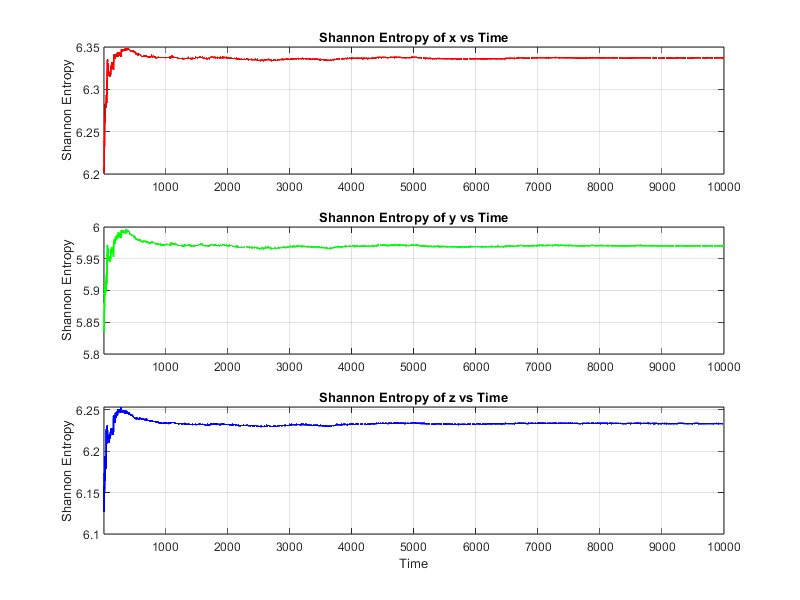
\includegraphics[width=0.8\linewidth]{SE_vs_time_x_y_z.png}
		\caption{Shanon Entropy over time}
		\label{SE_forx_time_series}
	\end{figure}
	
	\begin{figure}[htbp]
		\centering
		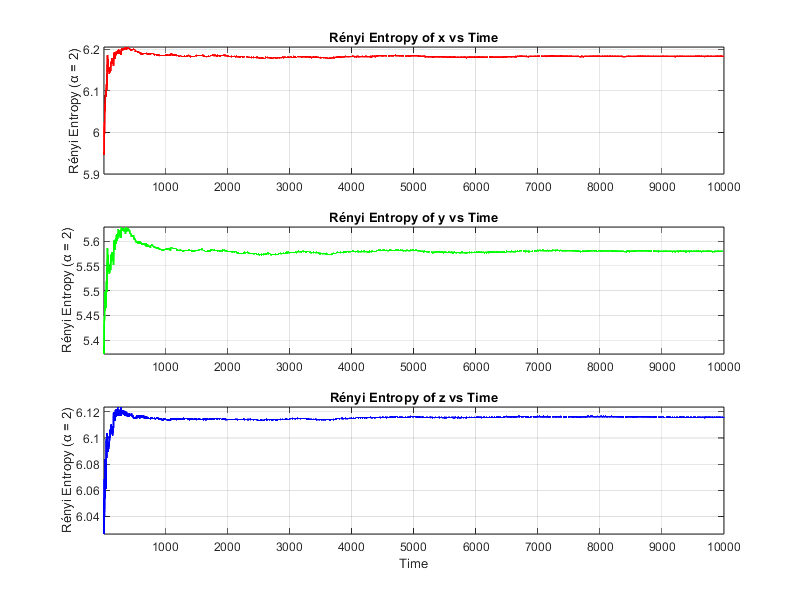
\includegraphics[width=0.8\linewidth]{RE_vs_time_x_y_z.png}
		\caption{Renyi Entropy over time}
		\label{fig:Renyi Entropy}
	\end{figure}
			\begin{figure}[htbp]
		\centering
		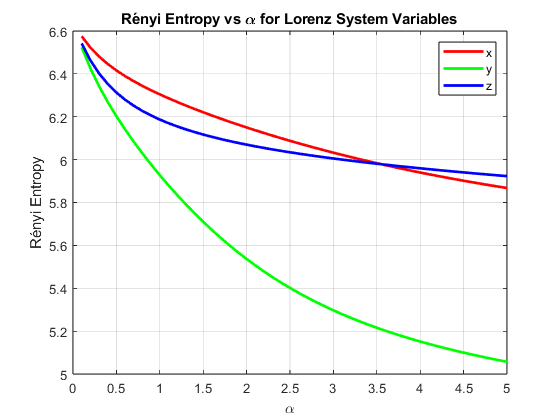
\includegraphics[width=0.8\linewidth]{renyi_entropy_vs_alpha_for_100_bin.png}
		\caption{Renyi Entropy with respect to $\alpha$}
		\label{fig:Renyi Entropy_alpha}
	\end{figure}
	\FloatBarrier

	\section{Conclusion}
	
	\begin{acknowledgments}
		We acknowledge helpful discussions with colleagues and support from our institutions. This work was supported by the XYZ Foundation (Grant No. 12345).
	\end{acknowledgments}
	
	\appendix
	\section{Technical Details}
	
	The appendix provides additional mathematical details omitted from the main text for readability.
	
	\begin{equation}
		\mathcal{R} = \sum_{i=1}^N \frac{x_i^2}{2\sigma^2}.
		\label{eq:appendix_eq}
	\end{equation}
	
	\bibliography{apssamp}
	
\end{document}
% ****** End of file apssamp.tex ******


\begin{acknowledgments}
	We wish to acknowledge the support of the author community in using
	REV\TeX{}, offering suggestions and encouragement, testing new versions,
	\dots.
\end{acknowledgments}

\appendix

\section{Appendixes}

\begin{verbatim}
	\appendix
	\section{}
\end{verbatim}
will produce an appendix heading that says ``APPENDIX A'' and
\begin{verbatim}
	\appendix
	\section{Background}
\end{verbatim}
will produce an appendix heading that says ``APPENDIX A: BACKGROUND''
(note that the colon is set automatically).

If there is only one appendix, then the letter ``A'' should not
appear. This is suppressed by using the star version of the appendix
command (\verb+\appendix*+ in the place of \verb+\appendix+).

\section{A little more on appendixes}

Observe that this appendix was started by using
\begin{verbatim}
	\section{A little more on appendixes}
\end{verbatim}

Note the equation number in an appendix:
\begin{equation}
	E=mc^2.
\end{equation}

\subsection{\label{app:subsec}A subsection in an appendix}


% The \nocite command causes all entries in a bibliography to be printed out
% whether or not they are actually referenced in the text. This is appropriate
% for the sample file to show the different styles of references, but authors
% most likely will not want to use it.
\nocite{*}
\bibliography{apssamp}% Produces the bibliography via BibTeX.

\end{document}
%
% ****** End of file apssamp.tex ******
